\chapter{Trees and Suslin's Problem} \label{Ch4:CH}
\thispagestyle{empty}

Suslin asked whether the real line is characterized by a condition weaker than separability, and the answer turns out to depend on the universe of sets. This chapter states the question and then develops the combinatorics that bears on it: trees, the tree property, and the principle $\Diamond$, from which we construct a Suslin tree.

\section{Suslin's Problem} \label{Ch4:Sec:Suslin}

We now put $L$ to work on a question about the real line which, on its face, has nothing to do with set theory.

\subsection{Dense Linear Orderings without Endpoints}

Here are some simple facts about dense linear orderings without endpoints. We should be able to prove these using prior knowledge.

We will abbreviate ``Dense Linear Ordering without Endpoints'' DLO (WE will be implicit).

\begin{boxlemma}
    Up to isomorphism, $\Q$ is the unique countable DLO.
\end{boxlemma}

As a reminder, this is a back-and-forth argument; if we have $\Q$ and another one, then we build an isomorphism by going back and forth.

The reals have a characterization of the same kind.

\begin{boxlemma}
    Up to isomorphism, $\R$ is the unique DLO that is separable (ie, admits a countable, dense subset) and complete (ie, has the least upper-bound property).
\end{boxlemma}

As a reminder, if $\parenth{\SS, <_{\SS}}$ is a DLO that's separable and complete, then we get an isomorphism between the dense countable subsets by the previous one, then using the LUB property, we extend that to an isomorphism on the entirety of the two sets.

Suslin's question is about a weakening of separability.

\begin{boxdefinition}[Countable Chain Condition]
    A DLO satisfies the \textbf{countable chain condition (CCC)} if every family of pairwise disjoint open intervals is countable.
\end{boxdefinition}

This is indeed weaker.

\begin{boxlemma}
    Every separable DLO satisfies the CCC.
\end{boxlemma}

\subsection{Suslin's Question}

Suslin asked the following question:
\begin{quote}
    Is every complete DLO satisfying the CCC isomorphic to $\R$?
\end{quote}
Suslin's Hypothesis says ``YES''. This is often abbreviated $\SH$. A counterexample to $\SH$ is called a Suslin Line. In other words, $\SH$ says that there are no Suslin lines.

Whether there are any turns out to depend on the universe of sets.

\begin{boxtheorem}[Jensen, 1960s]
    If $V = L$, then there exists a Suslin line.
\end{boxtheorem}

% [CORRECTED] was: ``$\SH$ holds in $L$'' --- Jensen's theorem gives a Suslin line in $L$, so it is $\neg\SH$ that holds there, which is what the corollary below needs
In other words, $\neg\SH$ holds in $L$. Since $L$ is a model of $\ZFC$ in which $V = L$ holds, the following is immediate.

\begin{boxcorollary}
    If $\ZFC$ is consistent, then so is $\ZFC \cup \set{\neg\SH}$.
\end{boxcorollary}

The other half cannot come from $L$, since $\SH$ fails there.

\begin{boxtheorem}[Solovay--Tennenbaum]
    If $\ZFC$ is consistent, then so is $\ZFC \cup \set{\SH}$.
\end{boxtheorem}

There is a name for a statement that a theory can neither prove nor refute.

\begin{boxdefinition}[Independence]
    Let $\Gamma$ be a theory and $\sigma$ a sentence. We say that $\sigma$ is \textbf{independent of $\Gamma$} if $\Gamma \nvdash \sigma$ and $\Gamma \nvdash \neg\sigma$, ie, if $\Gamma \cup \set{\sigma}$ and $\Gamma \cup \set{\neg\sigma}$ are both consistent.
\end{boxdefinition}

We thus say that $\SH$ is independent of $\ZFC$, as long as $\ZFC$ is consistent: by the corollary and the theorem above, $\ZFC \cup \set{\neg\SH}$ and $\ZFC \cup \set{\SH}$ are then both consistent.

\section{Trees}

So far, we've only looked at trees on $\omega$ or trees on some other set. These are subtrees of $\parenth{{^{<\omega}\Omega, \subsetneq}}$. Here is the general notion.

\begin{boxdefinition}[Tree]
    $\parenth{T, <_T}$ is a \textbf{tree} iff it's a strict partial ordering (transitive and irreflexive) and, for all $y \in T$, $\setst{x}{x <_T y}$ is well-ordered by $<_T$.
\end{boxdefinition}

Fix a tree $\parenth{T, <_T}$.

Each node of a tree sits at some height, and the nodes at the same height make up a level.

\begin{boxdefinition}[Height and Levels]
    For $y \in T$, define
    \begin{align*}
        \height_T(y) &= \type\of{\setst{x}{x <_T y}, <_T} \\
        \level_{\alpha}(T) &= \setst{y \in T}{\height_T(y) = \alpha} \\
        \height(T) &= \text{the least $\alpha$ such that $\level_{\alpha}(T) = \emptyset$}
    \end{align*}
    We call $\height_T(y)$ the \textbf{height} of $y$, $\level_{\alpha}(T)$ the \textbf{$\alpha$th level} of $T$, and $\height(T)$ the \textbf{height} of $T$.
\end{boxdefinition}

We will mostly care about trees that are as well-behaved as possible.

\begin{boxdefinition}[Normal Tree]
    We say $\parenth{T, <_T}$ is \textbf{normal} iff
    \begin{enumerate}
        \item $T$ has a unique root
        \item Splitting to the next level: given $x$ with $\height(x) = \alpha$, there are $y, z \in \level_{\alpha + 1}(T)$ such that $y \neq z$ and $x <_T y, z$.
        \begin{figure}[H]
            \centering
            \begin{tikzpicture}[dot/.style = {circle, fill, inner sep = 1.5pt}, every node/.style = {font = \small}]
                \draw[dashed, gray] (-2, 0) -- (2, 0) node[right, black] {$\level_{\alpha}(T)$};
                \draw[dashed, gray] (-2, 1.5) -- (2, 1.5) node[right, black] {$\level_{\alpha + 1}(T)$};
                \draw[dotted] (0, -1) -- (0, 0);
                \node[dot, label = {right:$x$}] (x) at (0, 0) {};
                \node[dot, label = {above:$y$}] (y) at (-0.8, 1.5) {};
                \node[dot, label = {above:$z$}] (z) at (0.8, 1.5) {};
                \draw (x) -- (y);
                \draw (x) -- (z);
            \end{tikzpicture}
        \end{figure}
        \item Extensions at every higher level: $\forall \alpha < \height(T)$, $\forall \beta$ with $\alpha < \beta < \height(T)$, $\forall x \in \level_{\alpha}(T)$, $\exists y \in \level_{\beta}(T)$ such that $x <_T y$.
        \item Extensionality at limit levels\footnote{so far, in homework, we've only seen trees with at most $\omega$ many levels; here, we're not assuming this of every tree}: given a limit ordinal $\alpha < \height(T)$, if $y, z \in \level_{\alpha}(T)$ and $\setst{x}{x <_T y} = \setst{x}{x <_T z}$, then $y = z$. So the following picture, in which $y \neq z$ sit on a limit level above exactly the same nodes, cannot occur in a normal tree.
        \begin{figure}[H]
            \centering
            \begin{tikzpicture}[dot/.style = {circle, fill, inner sep = 1.5pt}, every node/.style = {font = \small}]
                \foreach \h in {0, 1, 1.7, 2.15, 2.45}
                    \node[dot] at (0, \h) {};
                \draw (0, 0) -- (0, 2.45);
                \node at (0, 2.85) {$\vdots$};
                \draw[dashed, gray] (-2, 4) -- (2, 4) node[right, black] {$\level_{\alpha}(T)$, $\alpha$ limit};
                \node[dot, label = {above:$y$}] (y) at (-0.8, 4) {};
                \node[dot, label = {above:$z$}] (z) at (0.8, 4) {};
                \draw[dotted] (0, 3.2) -- (y);
                \draw[dotted] (0, 3.2) -- (z);
                \node[left, align = right] at (-0.3, 1.1) {$\setst{x}{x <_T y}$ \\ $= \setst{x}{x <_T z}$};
            \end{tikzpicture}
        \end{figure}
    \end{enumerate}
\end{boxdefinition}

Finally, branches are the paths through a tree, of any length.

\begin{boxdefinition}[Branch]
    A \textbf{branch} of a tree $\parenth{T, <_T}$ is a subset $b \subset T$ such that $\forall y \in b$, $\forall x <_T y$, $x \in b$ and $b$ is linearly ordered (equivalently, well-ordered) by $<_T$. We say $b$ is an \textbf{$\alpha$-branch} if $\type\of{b, <_T} = \alpha$.
\end{boxdefinition}

Two nodes of a tree may or may not lie on a common branch.

\begin{boxdefinition}[Comparability and Incomparability]
    Given a tree $T$, we say $x$ and $y$ are \textbf{comparable} (written $x \parallel y$) iff $x \leq_T y$ or $y \leq_T x$. Else, we say $x$ and $y$ are \textbf{incomparable} and write $x \perp y$.
\end{boxdefinition}

Sets of pairwise incomparable nodes will matter a great deal.

\begin{boxdefinition}[Antichain]
    $A \ssq T$ is an \textbf{antichain} (often abbreviated ac) if $\forall x, y \in A$, $x \neq y$ implies $x \perp y$.
\end{boxdefinition}

The levels are the basic example.

\begin{boxexample}
    For every $\alpha$, $\level_{\alpha}\of{T}$ is an antichain.
\end{boxexample}

An antichain may also be as large as possible.

\begin{boxdefinition}[Maximal Antichain]
    An antichain $A \ssq T$ in a tree $T$ is \textbf{maximal} iff
    \begin{enumerate}
        \item $A$ is an antichain
        \item There's no antichain $B$ with $B \supsetneq A$
    \end{enumerate}
\end{boxdefinition}

Note: if $A$ is a maximal antichain then for every $x \in T$, there's some $a \in A$ such that $a \parallel x$. Otherwise, $A \cup \set{x} = B$ would be an antichain.

% This file is the inbox for the lecture in progress. Type today's raw notes straight into
% it: it is \input from the chapter file, so the Overleaf preview builds them live. Once the
% material has been placed into the sections, /integrate empties the file again and leaves
% this header behind. Do not delete the file or its \input line.

\begin{boxdefinition}[$\lambda$-Tree]
    Let $\lambda$ be an infinite cardinal and $\parenth{T, <_T}$ be a tree. Then $T$ is a \textbf{$\lambda$-tree} iff $T$ has height $\lambda$ and $\forall \alpha < \lambda$, $\abs{\level_{\alpha}\of{T}} < \lambda$.
\end{boxdefinition}

The question is whether such a tree must have a branch running all the way up.

\begin{boxdefinition}[Tree Property]
    $\lambda$ has the \textbf{tree property} (often abbreviated TP) if every normal $\lambda$-tree has a $\lambda$-branch.
\end{boxdefinition}

The trees that witness a failure of the tree property have a name.

\begin{boxdefinition}[Aronszajn Tree]
    A \textbf{$\lambda$-Aronszajn Tree} (often abbreviated $\lambda$-A-tree) is a normal $\lambda$-tree with no $\lambda$-branch.
\end{boxdefinition}

Thus $\lambda$ has the TP iff there are no $\lambda$-A-trees. At the first two infinite cardinals, the answers go opposite ways.

\begin{boxtheorem}[K\H{o}nig]
    $\omega$ has the TP.
\end{boxtheorem}

\begin{boxtheorem}[Aronszajn]
    $\omega_1$ does \textit{not} have the TP.
\end{boxtheorem}

Proofs can be found in Ernest's book~\cite[Theorems 5.17 and 5.30]{Schimmerling} and in Kunen~\cite[Chapter II, Lemma 5.7 and Theorem 5.9]{Kunen}.

\begin{boxdefinition}[Comparability and Incomparability]
    Given a tree $T$, we say $x$ and $y$ are \textbf{comparable} (written $x \parallel y$) iff $x \leq_T y$ or $y \leq_T x$. Else, we say $x$ and $y$ are \textbf{incomparable} and write $x \perp y$.
\end{boxdefinition}

\begin{boxdefinition}[Antichain]
    $A \ssq T$ is an \textbf{antichain} (often abbreviated ac) if $\forall x, y \in A$, $x \neq y$ implies $x \perp y$.
\end{boxdefinition}

\begin{boxexample}
    For every $\alpha$, $\level_{\alpha}\of{T}$ is an antichain.
\end{boxexample}

% fill in from phone pictures

% state jensen's theorem

\begin{boxdefinition}[$\Diamond$]
    Let $\lambda$ be a regular, uncountable cardinal. Let $E \ssq \lambda$. We define \textbf{$\Diamond_{\lambda}(E)$} to be the statement that there is some sequence $\grpres{A_{\alpha}}{\alpha \in E}$ such that the following both hold:
    \begin{enumerate}
        \item Each $A_{\alpha}$ is a subset of $\alpha$
        \item For every $X \ssq \lambda$, the set $S_X = \setst{\alpha \in E}{\alpha \cap X = A_{\alpha}}$ is a stationary subset of $\lambda$.
    \end{enumerate}
    $\Diamond_{\lambda}(E)$ is shorthand the statement that there is a $\Diamond_{\lambda}(E)$-sequence, and $\Diamond_{\lambda}$ is shorthand for the statement that there is a $\Diamond_{\lambda}(\lambda)$-sequence.
\end{boxdefinition}

\begin{boxproposition}[Properties of $\Diamond$]\hfill
    \begin{enumerate}
        \item $\Diamond_{\lambda} \equiv \Diamond_{\lambda}(\lambda)$
        \item $\Diamond(E) \equiv  \Diamond_{\omega_1}(E)$
        \item $\Diamond \equiv \Diamond_{\omega_1}\of{\omega_1} = \Diamond_{\omega_1}$
    \end{enumerate}
\end{boxproposition}

\begin{boxlemma}
    Suppose $X$ is a bounded subset of $\lambda$ (so we have $\beta < \lambda$ such that $X \ssq \beta$). Assume $\grpres{A_{\alpha}}{\alpha < \lambda}$ is a $\Diamond_{\lambda}$-sequence. Then $\setst{\alpha < \lambda}{A_{\alpha} = X}$ is stationary in $\lambda$.
\end{boxlemma}

\begin{boxcorollary}
    $\Diamond_{\lambda} \to 2^{<\lambda} = \lambda$.
\end{boxcorollary}

In particular, when $\lambda = \omega_1$, we have $2^{< \omega_1} = 2^{\omega} = \omega_1$, so CH holds. In other words, diamond implies CH.

\begin{boxlemma}
    Assume $\Diamond_{\lambda}(E)$. Then $\grpres{S_X}{X \ssq \lambda}$ (where $S_X$ is defined from the witness to $\Diamond_{\lambda}(E)$) splits $E$ into $2^{\lambda}$ many almost disjoint pieces. This could mean:
    \begin{itemize}
        \item For $X \neq Y$ both subsets of $\lambda$, $S_X \cap S_Y$ is bounded in $\lambda$
        \item For $X \neq Y$ both subsets of $\lambda$, $S_X \cap S_Y$ is non-stationary in $\lambda$.
    \end{itemize}
\end{boxlemma}
\begin{proof}
    For $X \neq Y$, take $\beta = \min(X \symmdiff Y) < \lambda$. Then, for $\alpha > \beta$, $X \cap \alpha \neq Y \cap \alpha$. So we can't have $X \cap \alpha = A_{\alpha}$ and $Y \cap \alpha  = A_{\alpha}$.
\end{proof}

Recall the Solovay Splitting Theorem.

\begin{boxtheorem}[Solovay Splitting Theorem]
    Given $E \ssq \lambda$ stationary, with $\lambda = \cf(\lambda) > \omega$, we can partition $E$ into $\lambda$ many pieces, each of which is stationary.
\end{boxtheorem}

\begin{boxlemma}
    $\parenth{T, <_{T}}$ is a Souslin tree iff it's a normal $\omega_1$-tree with no uncountable antichain.
\end{boxlemma}

\begin{boxdefinition}[Maximal Antichain]
    An antichain $A \ssq T$ in a tree $T$ is \textbf{maximal} iff
    \begin{enumerate}
        \item $A$ is an antichain
        \item There's no antichain $B$ with $B \supsetneq A$
    \end{enumerate}
\end{boxdefinition}

Note: if $A $is a maximal antichain then for every $x \in T$, there's some $a \in A$ such that $a \parallel x$. Otherwise, $A \cup \set{x} = B$ would be an antichain.

\begin{boxconstruction}[Constructing a Souslin Tree from a Diamond]
    Fix a $\Diamond$-sequence $\grpres{A_{\alpha}}{\alpha < \omega_1}$. By recursion, we'll build trees $\parenth{T_{\alpha}, <_{\alpha}}$ indexed by ordinals $\alpha < \omega_1$. We'll maintain:
    \begin{enumerate}
        \item $T_{\alpha}$ is a tree of height $\alpha$
        \item $T_{\alpha}$ as a set (not as a tree) is a countable ordinal. In fact, $\alpha \leq T_{\alpha} < \omega_1$
        \item For $\alpha < \beta < \omega_1$, $T_{\alpha}$ is end-extended by $T_{\beta}$ (trees) in the ``strong sense'':
        \begin{enumerate}
            \item $<_{\alpha} \ssq <_{\beta}$
            \item for every $\eta < \alpha$, $\level_{\eta}\of{T_{\alpha}} = \level_{\eta}\of{T_{\beta}}$
        \end{enumerate}
    \end{enumerate}
    The plan is to define $\parenth{T, <_T}$ to be the union of the $\parenth{T_{\alpha}, <_{\alpha}}$s and get that $\parenth{T, <_T}$ is a Souslin-tree, but other things need to hold for this. \\

    Consider the base case
    \begin{align*}
        \parenth{T_0, <_0} = \parenth{0, \emptyset}
    \end{align*}
    Define $\parenth{T_1, <_1} := \parenth{\set{0}, \emptyset}$. We want to define $T_2$ to be the tree with root $0$ and children $1$ and $2$. Or something like that. So define
    \begin{align*}
        \parenth{T_2, <_2} := \parenth{\set{0, 1, 2}, \set{(0, 1), (0, 2)}}
    \end{align*}
    \begin{figure}[H]
        \centering
        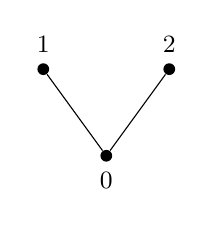
\begin{tikzpicture}[dot/.style = {circle, fill, inner sep = 1.5pt}, every node/.style = {font = \small}, grow' = up, level distance = 1.1cm, sibling distance = 1.6cm]
            \node[dot, label = {below:$0$}] {}
                child {node[dot, label = {above:$1$}] {}}
                child {node[dot, label = {above:$2$}] {}};
        \end{tikzpicture}
    \end{figure}
    In similar fashion, we define $T_3$ to be the tree extending $T_2$ with the children of $1$ being $3$ and $4$ and the children of $2$ being $5$ and $6$.
    \begin{figure}[H]
        \centering
        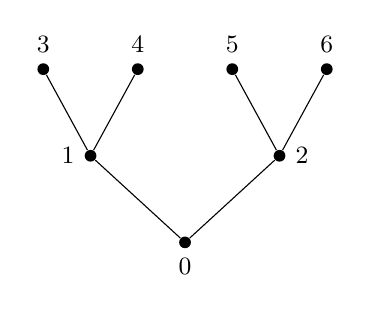
\begin{tikzpicture}[dot/.style = {circle, fill, inner sep = 1.5pt}, every node/.style = {font = \small}, grow' = up, level distance = 1.1cm, level 1/.style = {sibling distance = 2.4cm}, level 2/.style = {sibling distance = 1.2cm}]
            \node[dot, label = {below:$0$}] {}
                child {node[dot, label = {left:$1$}] {}
                    child {node[dot, label = {above:$3$}] {}}
                    child {node[dot, label = {above:$4$}] {}}}
                child {node[dot, label = {right:$2$}] {}
                    child {node[dot, label = {above:$5$}] {}}
                    child {node[dot, label = {above:$6$}] {}}};
        \end{tikzpicture}
    \end{figure}
    This is how we define successor trees. \\

    % Transcribed from the board photographs.
    % [CORRECTED] was: ``can be listed as $\xi_n$ for $n < \omega$'' and ``is $T_{\gamma} + \omega$'', for every $\beta$ --- when $\beta$ is finite the level has $2^{\beta}$ nodes and $T_{\delta} = T_{\gamma} + 2^{\beta + 1}$ (eg $T_3 = 7$, not $\omega$)
    Now consider the successor of a successor level. Say $\delta = \gamma + 1 = \parenth{\beta + 1} + 1$. How do we define $\parenth{T_{\delta}, <_{\delta}}$ based on $\parenth{T_{\gamma}, <_{\gamma}}$? We know (by the recursion hypothesis) that the universe of $T_{\gamma}$ is a countable ordinal. So $\level_{\beta}\of{T_{\gamma}}$ can be listed as $\xi_n$ for $n < \omega$ (for $n < 2^{\beta}$, if $\beta$ is finite). Define $T_{\delta}$ by putting $T_{\gamma} + 2n$ and $T_{\gamma} + 2n + 1$ above $\xi_n$.
    \begin{figure}[H]
        \centering
        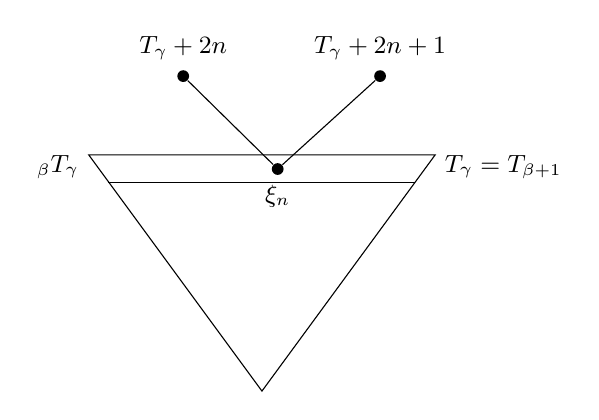
\begin{tikzpicture}[dot/.style = {circle, fill, inner sep = 1.5pt}, every node/.style = {font = \small}]
            \draw (0, 0) -- (-2.2, 3) -- (2.2, 3) -- cycle;
            \draw (-1.95, 2.65) -- (1.95, 2.65);
            \node[left] at (-2.2, 2.85) {$\level_{\beta}\of{T_{\gamma}}$};
            \node[right] at (2.2, 2.85) {$T_{\gamma} = T_{\beta + 1}$};
            \node[dot, label = {below:$\xi_n$}] (x) at (0.2, 2.82) {};
            \node[dot, label = {above:$T_{\gamma} + 2n$}] (y) at (-1, 4) {};
            \node[dot, label = {above:$T_{\gamma} + 2n + 1$}] (z) at (1.5, 4) {};
            \draw (x) -- (y);
            \draw (x) -- (z);
        \end{tikzpicture}
    \end{figure}
    We see that $T_{\delta}$ (the universe) is $T_{\gamma} + \omega$ (or $T_{\gamma} + 2^{\beta + 1}$, if $\beta$ is finite, as with $T_2$ and $T_3$). \\

    At every limit ordinal $\beta < \omega_1$, define
    \begin{align*}
        \parenth{T_{\beta}, <_{\beta}} := \parenth{\bigcup_{\alpha < \beta} T_{\alpha}, \bigcup_{\alpha < \beta} <_{\alpha}}
    \end{align*}
    In particular, we now know $\parenth{T_{\omega}, <_{\omega}}$. It's easy to see that $\parenth{T_{\omega}, <_{\omega}} \simeq {^{<\omega}2}$.

    % Transcribed from the board photographs.
    All that remains is
    \begin{enumerate}
        \item how to define $\parenth{T_{\delta}, <_{\delta}}$ when $\delta = \gamma + 1$ and $\gamma$ is a limit ordinal, and
        \item why it works.
    \end{enumerate}
\end{boxconstruction}
